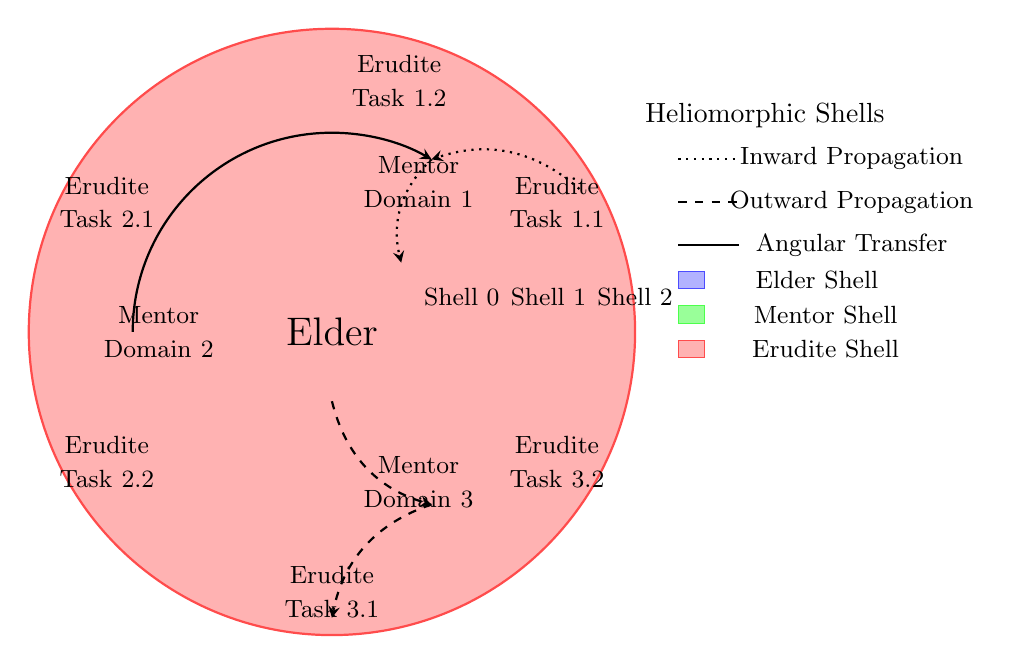
\begin{tikzpicture}[scale=1.1]
  % Define colors
  \colorlet{eldershell}{blue!30}
  \colorlet{mentorshell}{green!40}
  \colorlet{eruditeshell}{red!30}
  \colorlet{elderborder}{blue!70}
  \colorlet{mentorborder}{green!70}
  \colorlet{eruditeborder}{red!70}
  
  % Draw concentric circles for shells
  \draw[fill=eldershell, draw=elderborder, thick] (0,0) circle (1.5);
  \draw[fill=mentorshell, draw=mentorborder, thick] (0,0) circle (2.5);
  \draw[fill=eruditeshell, draw=eruditeborder, thick] (0,0) circle (3.5);
  
  % Add Elder, Mentor, Erudite labels
  \node at (0,0) {\Large Elder};
  
  % Mentor text nodes at different angles
  \node[text width=1.5cm, align=center] at (60:2) {\small Mentor\\Domain 1};
  \node[text width=1.5cm, align=center] at (180:2) {\small Mentor\\Domain 2};
  \node[text width=1.5cm, align=center] at (300:2) {\small Mentor\\Domain 3};
  
  % Erudite text nodes at different angles
  \node[text width=1.5cm, align=center] at (30:3) {\small Erudite\\Task 1.1};
  \node[text width=1.5cm, align=center] at (75:3) {\small Erudite\\Task 1.2};
  \node[text width=1.5cm, align=center] at (150:3) {\small Erudite\\Task 2.1};
  \node[text width=1.5cm, align=center] at (210:3) {\small Erudite\\Task 2.2};
  \node[text width=1.5cm, align=center] at (270:3) {\small Erudite\\Task 3.1};
  \node[text width=1.5cm, align=center] at (330:3) {\small Erudite\\Task 3.2};
  
  % Arrows for Knowledge Flow
  % Inward propagation (abstraction)
  \draw[->, thick, dotted, >=stealth, draw=black] (30:3.3) to[bend right] (60:2.3);
  \draw[->, thick, dotted, >=stealth, draw=black] (60:2.3) to[bend right] (0.8,0.8);
  
  % Outward propagation (specialization)
  \draw[->, thick, dashed, >=stealth, draw=black] (0,-0.8) to[bend right] (300:2.3);
  \draw[->, thick, dashed, >=stealth, draw=black] (300:2.3) to[bend right] (270:3.3);
  
  % Angular dynamics (cross-domain transfer)
  \draw[->, thick, >=stealth, draw=black] (180:2.3) arc (180:60:2.3);
  
  % Legend
  \node[align=left] at (5,2.5) {Heliomorphic Shells};
  \draw[thick, dotted, >=stealth, draw=black] (4,2) -- (4.7,2);
  \node[align=left, font=\small] at (6,2) {Inward Propagation};
  \draw[thick, dashed, >=stealth, draw=black] (4,1.5) -- (4.7,1.5);
  \node[align=left, font=\small] at (6,1.5) {Outward Propagation};
  \draw[thick, >=stealth, draw=black] (4,1) -- (4.7,1);
  \node[align=left, font=\small] at (6,1) {Angular Transfer};
  
  \draw[fill=eldershell, draw=elderborder] (4,0.5) rectangle (4.3,0.7);
  \node[align=left, font=\small] at (5.6,0.6) {Elder Shell};
  \draw[fill=mentorshell, draw=mentorborder] (4,0.1) rectangle (4.3,0.3);
  \node[align=left, font=\small] at (5.7,0.2) {Mentor Shell};
  \draw[fill=eruditeshell, draw=eruditeborder] (4,-0.3) rectangle (4.3,-0.1);
  \node[align=left, font=\small] at (5.7,-0.2) {Erudite Shell};
  
  % Shell indices
  \node[font=\small] at (1.5,0.4) {Shell 0};
  \node[font=\small] at (2.5,0.4) {Shell 1};
  \node[font=\small] at (3.5,0.4) {Shell 2};
\end{tikzpicture}